\begin{mdframed}[backgroundcolor=red!5]
This work is part of the MSc thesis of T. Weir (2018).
\end{mdframed}

We first start with an isothermal Stokes flow, so that we disregard the heat transport equation and 
the equations we wish to solve are simply:

\begin{align}
  \label{eq:stokes-1}
  -\nabla \cdot \left[2\eta \left(\dot\varepsilon(\bm v)
                                  - \frac{1}{3}(\nabla \cdot \bm v)\mathbf 1\right)
                \right] + \nabla p &=
  \rho \bm g
  &
  & \textrm{in $\Omega$},
  \\
  \label{eq:stokes-2}
  \nabla \cdot (\rho \bm v) &= 0
  &
  & \textrm{in $\Omega$}
\end{align}
The second equation can be rewritten 
$\nabla \cdot (\rho {\bm v}) =  \rho \nabla \cdot {\bm v} + {\bm v} \cdot {\bm \nabla}\rho=0$
or, 
\[
\nabla \cdot {\bm v} + \frac{1}{\rho} {\bm v} \cdot {\bm \nabla}\rho=0
\]
Note that this presupposes that the density is not zero anywhere in the domain.

We use a mixed formulation and therefore  
keep both velocity and pressure as unknowns. We end up having to solve 
the following system:
\[
\left(
\begin{array}{cc}
\K & \G \\ \G^T+\Z & 0 
\end{array}
\right)
\cdot
\left(
\begin{array}{c}
{\cal V} \\ {\cal P}
\end{array}
\right)
=
\left(
\begin{array}{c}
 f \\ h
\end{array}
\right)
\quad\quad
{\rm or,}
\quad\quad
\A \cdot X = rhs
\]
Where $\K$ is the stiffness matrix, $\G$ is the discrete gradient operator, 
$\G^T$ is the discrete divergence operator, ${\cal V}$ the velocity vector, 
${\cal P}$ the pressure vector.
Note that the term $\Z{\cal V}$ derives from term ${\bm v} \cdot {\bm \nabla} \rho$ in the continuity equation. 

Each block $\K$, $\G$ , $\Z$ and vectors $f$ and $h$ are built separately 
in the code and assembled into 
the matrix $\A$ and vector $rhs$ afterwards. $\A$ and $rhs$ are then passed to the solver. 
We will see later that there are alternatives to solve this approach which do not require to 
build the full Stokes matrix $\A$. 

{\sl Remark}: the term $\Z {\cal V}$ is often put in the rhs (i.e. added to $h$) so that 
the matrix $\A$ retains the same structure as in the incompressible case. This is indeed 
how it is implemented in ASPECT. This however requires more work since the rhs depends 
on the solution and some form of iterations is needed. 

In the case of a compressible flow the strain rate tensor and the deviatoric strain rate tensor are no more equal (since ${\bm \nabla}\cdot{\bm v} \neq 0$).
The deviatoric strainrate tensor is given by\footnote{See the ASPECT manual for a justification of the 3 value in the denominator in 2D and 3D.} 
\[
\dot{\bm \epsilon}^d({\bm v})=
\dot{\bm \epsilon}({\bm v})-\frac{1}{3} Tr(\dot{\bm \epsilon}) {\bm 1}
=\dot{\bm \epsilon}({\bm v})-\frac{1}{3} ({\bm \nabla}\cdot{\bm v}) {\bm 1}
\]
In that case:
\begin{eqnarray}
\dot{\epsilon}_{xx}^d 
&=& \frac{\partial u}{\partial x}
-\frac{1}{3} \left( \frac{\partial u}{\partial x} + \frac{\partial v}{\partial y} \right) 
= \frac{2}{3}\frac{\partial u}{\partial x}
-\frac{1}{3} \frac{\partial v}{\partial y}
%=
%\frac{2}{3} \sum_{i=1}^4 \frac{\partial N_i}{\partial x}\;  u_i 
%-\frac{1}{3} \sum_{i=1}^4 \frac{\partial N_i}{\partial y}\;  v_i 
\\
\dot{\epsilon}_{yy}^d 
&=& \frac{\partial v}{\partial y}
-\frac{1}{3} \left( \frac{\partial u}{\partial x} + \frac{\partial v}{\partial y} \right) 
=-\frac{1}{3} \frac{\partial u}{\partial x} 
+ \frac{2}{3} \frac{\partial v}{\partial y} 
%=-\frac{1}{3}  \sum_{i=1}^4 \frac{\partial N_i}{\partial x}\;  u_i
%+ \frac{2}{3} \sum_{i=1}^4 \frac{\partial N_i}{\partial y}\;  v_i
\\
2\dot{\epsilon}_{xy}^d 
&=& 
\frac{\partial u}{\partial y} 
+\frac{\partial v}{\partial x} 
%= \sum_{i=1}^4 \frac{\partial N_i}{\partial y}\;  u_i
%+ \sum_{i=1}^4 \frac{\partial N_i}{\partial x}\;  v_i
\end{eqnarray}
and then 
\[
\dot{\bm \epsilon}^d({\bm v})
=
\left(
\begin{array}{cc}
\frac{2}{3} \frac{\partial u}{\partial x} -\frac{1}{3} \frac{\partial v}{\partial y} &
\frac{1}{2}\frac{\partial u}{\partial y} + \frac{1}{2}\frac{\partial v}{\partial x}  \\ \\
\frac{1}{2}\frac{\partial u}{\partial y} + \frac{1}{2}\frac{\partial v}{\partial x}  &
-\frac{1}{3} \frac{\partial u}{\partial x} +\frac{2}{3} \frac{\partial v}{\partial y} 
\end{array}
\right)
\]

From $\vec{\tau} = 2\eta \vec{\epsilon}^d$ we arrive at:
\[
\left(
\begin{array}{c}
\tau_{xx}\\
\tau_{yy}\\
\tau_{xy}\\
\end{array}
\right)
=
2\eta
\left(
\begin{array}{c}
\dot{\epsilon}_{xx}^d \\
\dot{\epsilon}_{yy}^d \\
\dot{\epsilon}_{xy}^d 
\end{array}
\right)
=2 \eta
\left(
\begin{array}{ccc}
2/3 & -1/3& 0 \\
-1/3 & 2/3 & 0 \\
0 & 0 & 1/2 \\
\end{array}
\right)
\cdot 
\left(
\begin{array}{c}
\frac{\partial u}{\partial x} \\ 
\frac{\partial v}{\partial y} \\ 
\frac{\partial u}{\partial y}\! +\! \frac{\partial v}{\partial x} \\
\end{array}
\right)
=
\eta
\left(
\begin{array}{ccc}
4/3 & -2/3& 0 \\
-2/3 & 4/3 & 0 \\
0 & 0 & 1 \\
\end{array}
\right)
\cdot 
\left(
\begin{array}{c}
\frac{\partial u}{\partial x} \\ 
\frac{\partial v}{\partial y} \\ 
\frac{\partial u}{\partial y}\! +\! \frac{\partial v}{\partial x} \\
\end{array}
\right)
\]
or, 
\[
\vec{\tau} = {\bm C}_\eta {\bm B} V
\]


















\newpage
In order to test our implementation we have created a few manufactured solutions:
\begin{itemize}
\item \underline{benchmark \#1} ({\tt ibench=1})): Starting from a density profile of:
\begin{equation}
    \rho(x,y) = xy
\end{equation}
We derive a velocity given by:
\begin{equation}
    v_x(x,y) = \frac{C_x}{x} , v_y(x,y) = \frac{C_y}{y}
\end{equation}

With $g_x(x,y) = \frac{1}{x}$ and $g_y(x,y) = \frac{1}{y}$, this leads us to a pressure profile:
\begin{equation}
    p = - \eta \left( \frac{4C_x}{3x^2} + \frac{4C_y}{3y^2} \right)  + xy + C_0
\end{equation}
This gives us a strain rate:
\[
\dot{\epsilon}_{xx} =  \frac{-C_x}{x^2}
\quad
\quad
\quad
\dot{\epsilon}_{yy} =  \frac{-C_y}{y^2}
\quad
\quad
\quad
\dot{\epsilon}_{xy} = 0 
\]
In what follows, we choose $\eta=1$ and $C_x=C_y=1$ and for a unit square domain $
[1:2]\times[1:2]$ we compute $C_0$
so that the pressure is normalised to zero over the whole domain and obtain $C_0=-1$. 
 
\item \underline{benchmark \#2} ({\tt ibench=2}): Starting from a density profile of:
\begin{equation}
    \rho = \cos(x)\cos(y)
\end{equation}
We derive a velocity given by:
\begin{equation}
    v_x = \frac{C_x}{\cos(x)} , v_y = \frac{C_y}{\cos(y)}
\end{equation}
With $g_x = \frac{1}{\cos(y)}$ and $g_y = \frac{1}{\cos(x)}$, this leads us to a pressure profile:
\begin{equation}
    p =  \eta \Bigg(\frac{4C_x \sin(x)}{3\cos^2(x)} + \frac{4C_y \sin(y)}{3\cos^2(y)}\Bigg) 
    +( \sin(x) + \sin(y) ) + C_0
\end{equation}
\[
\dot{\epsilon}_{xx} = C_x \frac{\sin(x)}{\cos^2(x)}
\quad
\quad
\quad
\dot{\epsilon}_{yy} = C_y \frac{\sin(y)}{\cos^2(y)}
\quad
\quad
\quad
\dot{\epsilon}_{xy} = 0 
\]
We choose $\eta=1$ and $C_x=C_y=1$. The domain is the unit square $[0:1]\times[0:1]$ and we obtain 
$C_0$ as before and obtain 
\[
C_0 = 2 - 2 \cos(1) + 8/3 (\frac{1}{\cos (1)} - 1)
\simeq 3.18823730
\]
(thank you WolframAlpha)


\item \underline{benchmark \#3} ({\tt ibench=3}) 
\item \underline{benchmark \#4} ({\tt ibench=4}) 
\item \underline{benchmark \#5} ({\tt ibench=5}) 
\end{itemize}




\fbox{
\parbox{10cm}{{\bf features}
\begin{itemize}
\item $Q_1\times P_0$ element \index{$Q_1 \times P_0$}
\item incompressible flow \index{incompressible flow}
\item mixed formulation \index{mixed formulation}
\item Dirichlet boundary conditions (no-slip)
\item isothermal \index{isothermal}
\item isoviscous \index{isoviscous}
\item analytical solution \index{analytical solution}
\item pressure smoothing \index{pressure smoothing} 
\end{itemize}
}}

%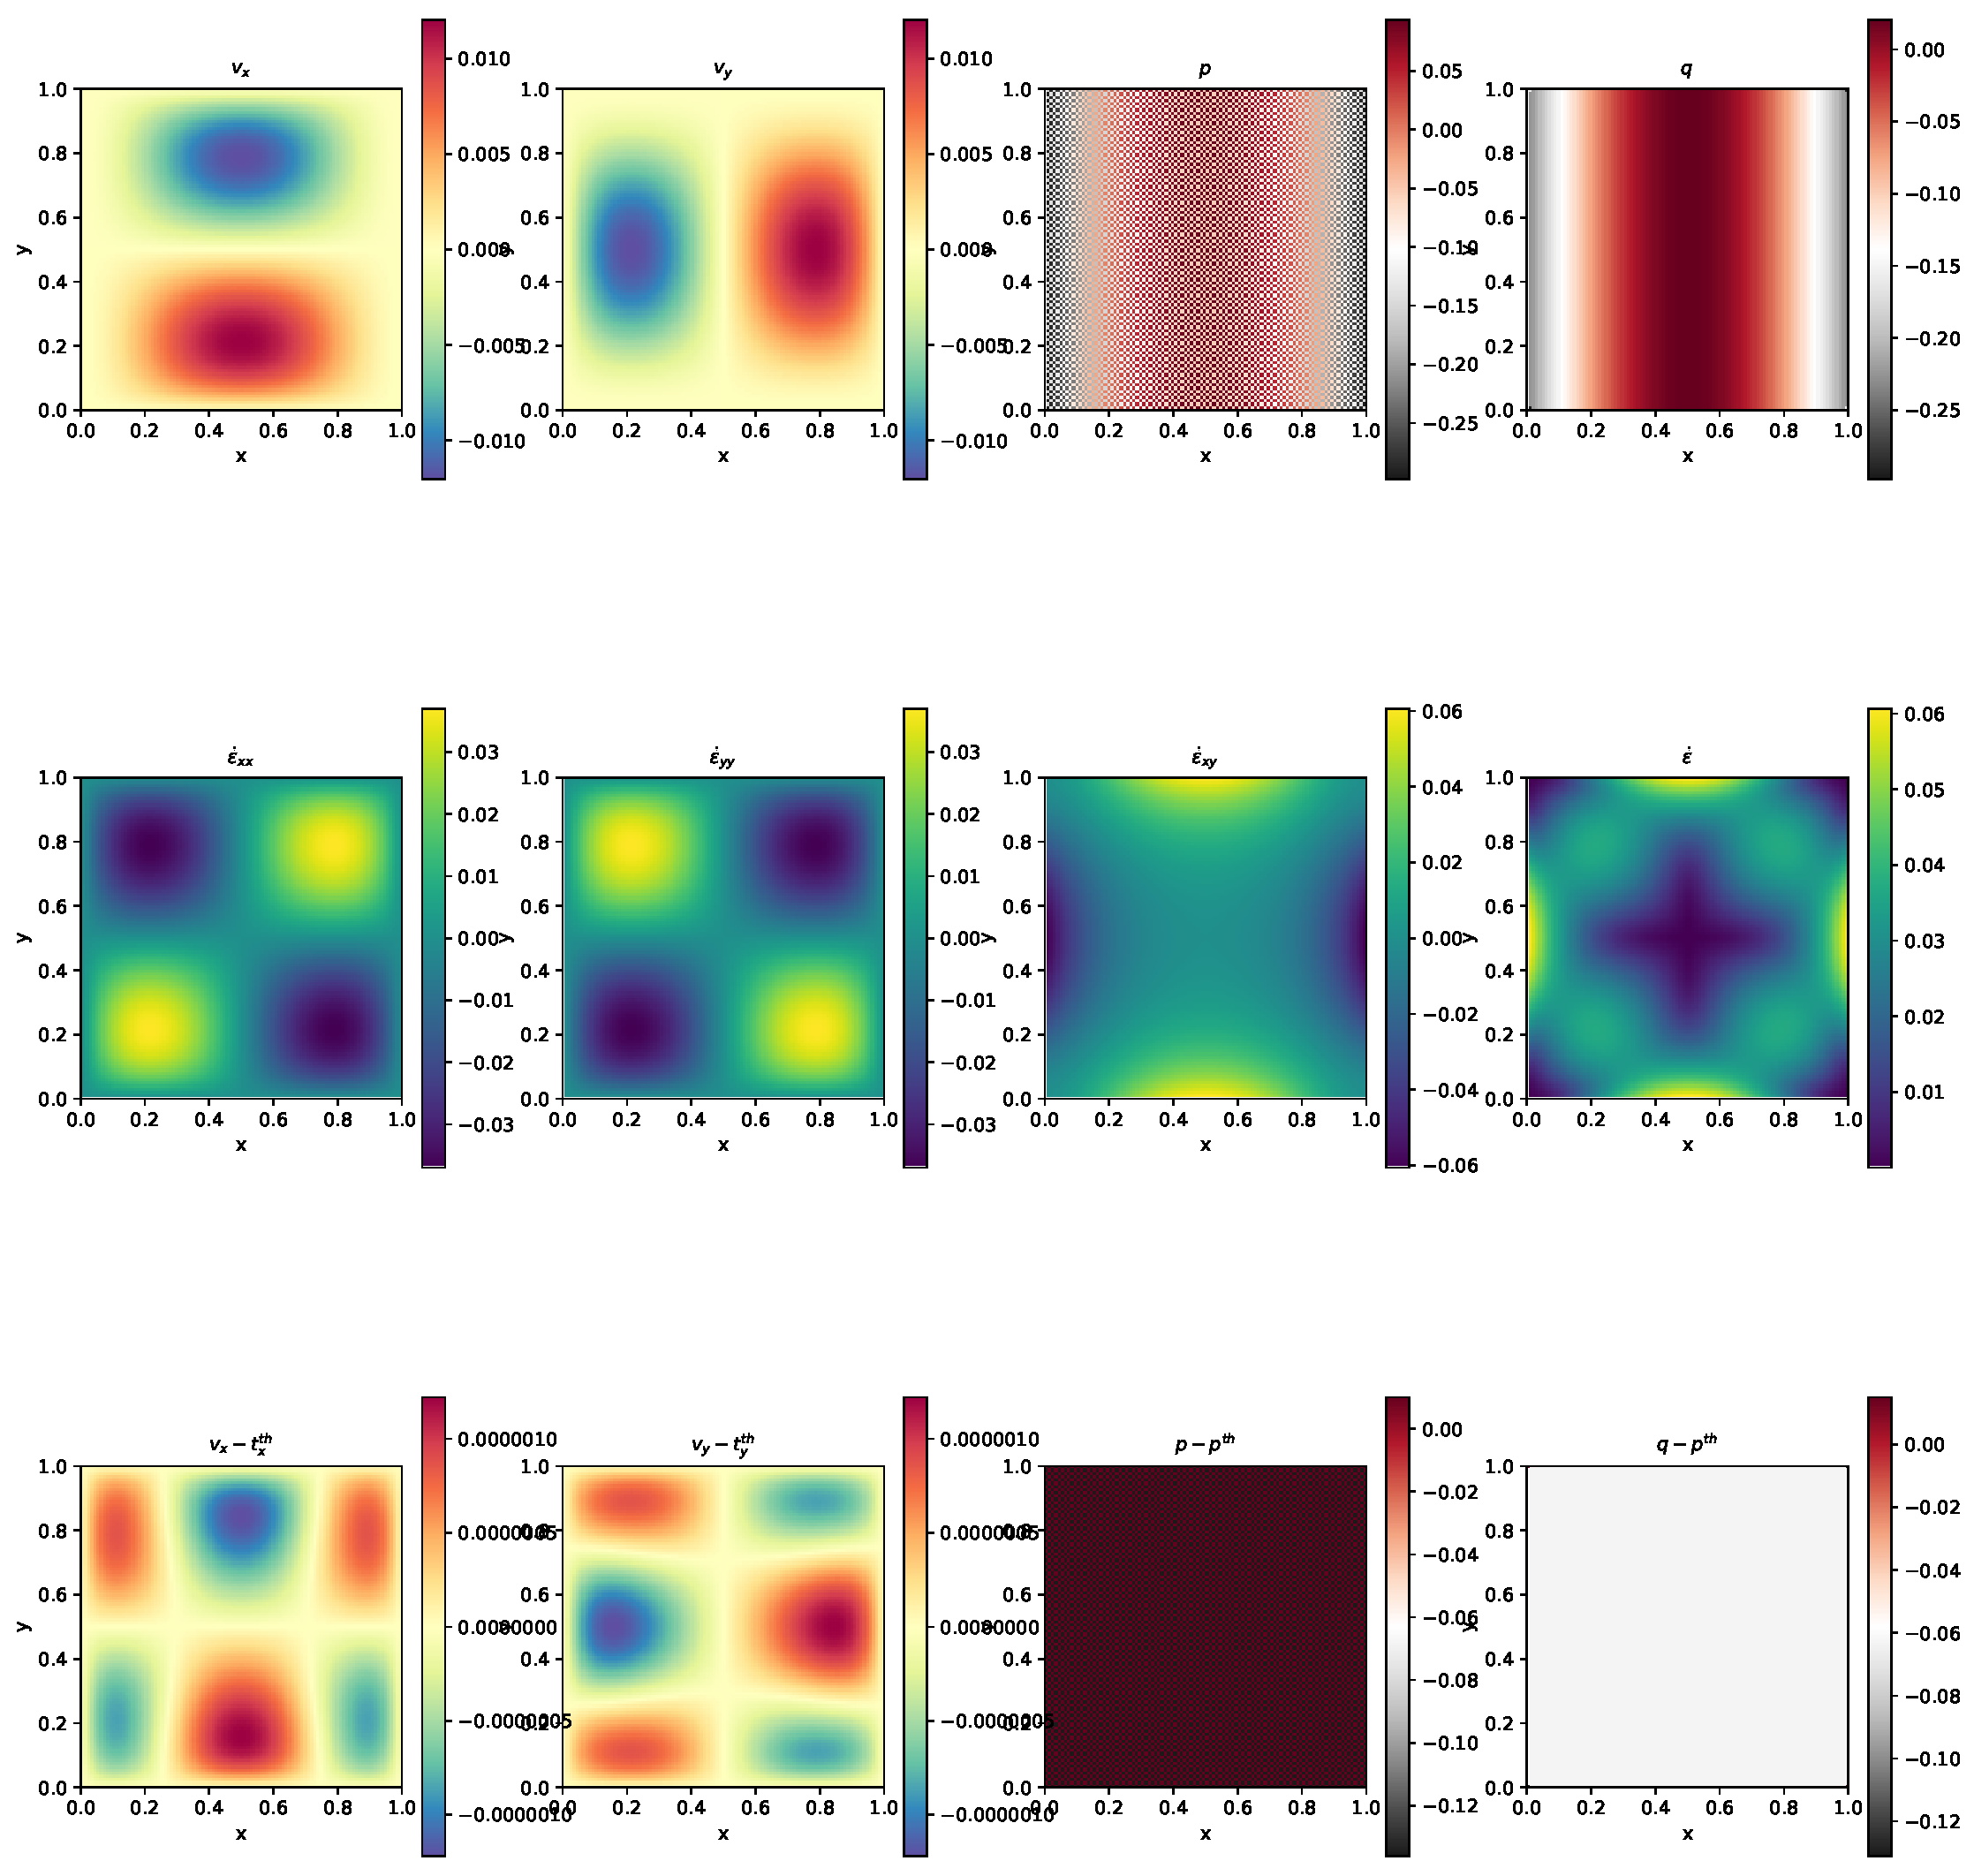
\includegraphics[width=16cm]{python_codes/fieldstone_saddlepoint/solution.pdf}

ToDo:
\begin{itemize}
\item pbs with odd vs even number of elements 
\item q is 'fine' everywhere except in the corners - revisit pressure smoothing paper?
\item redo A v d Berg benchmark (see Tom Weir thesis)
\end{itemize}


